\documentclass[12pt,a4paper]{article}

\usepackage[utf8]{inputenc}
\usepackage[T1]{fontenc}
\usepackage[brazil]{babel}
\usepackage{lmodern}
\usepackage{indentfirst}
\usepackage[dvipsnames]{xcolor}
\usepackage{graphicx}
\usepackage{amsmath}
\usepackage{textcomp}
\usepackage{booktabs}
\usepackage[hidelinks]{hyperref}
\usepackage[
	backend=biber,
	style=numeric,
	sorting=none
]{biblatex}
\addbibresource{referencias.bib}

% Margens ABNT (3cm esq/topo, 2cm dir/baixo) via primitivos do LaTeX,
% sem o pacote geometry - a versao instalada deste MiKTeX (2021, nunca
% atualizado) tem o kernel LaTeX2e desatualizado para pacotes recentes
% como geometry/siunitx, que agora exigem primitivos de 2022+.
\setlength{\oddsidemargin}{0.46cm}   % 3cm - 1in
\setlength{\evensidemargin}{0.46cm}
\setlength{\topmargin}{-0.54cm}      % 3cm - 1in - cabecalho padrao
\setlength{\headheight}{15pt}
\setlength{\headsep}{0.45cm}
\setlength{\textwidth}{16cm}       % 21cm - 3cm - 2cm
\setlength{\textheight}{23.85cm}      % 29.7cm - 3cm - 2cm (aprox.)

% Espacamento 1,5 (equivalente ao setspace) sem depender do pacote
\renewcommand{\baselinestretch}{1.5}

% Notas de fonte abaixo de figuras/tabelas (equivalente ao \legend do abntex2)
\newcommand{\legend}[1]{\par\vspace{2pt}\footnotesize #1}
% Citacao no estilo autor(2021) usada no texto corrido
\newcommand{\citeonline}[1]{\citeauthor{#1} (\citeyear{#1})}
\newcommand{\unbblue}{RoyalBlue}
\hypersetup{pdftitle={Projeto e Simulacao de um Ressonador Omega de Micro-ondas}, pdfsubject={Relatorio Tecnico de Projeto -- Universidade de Brasilia}, pdfkeywords={ODMR, centros NV, ressonador omega, micro-ondas, UnB}}
\makeatletter
\def\ps@unb{
  \def\@oddhead{\hfil\footnotesize\color{\unbblue}Universidade de Bras\'ilia -- Faculdade de Tecnologia\hfil}
  \def\@evenhead{\@oddhead}
  \def\@oddfoot{\hfil\footnotesize\thepage\hfil}
  \def\@evenfoot{\@oddfoot}
}
\makeatother
\pagestyle{unb}
\setcounter{tocdepth}{2}

\begin{document}
\hypersetup{pageanchor=false}

% --- Capa / folha de rosto (formatacao ABNT manual) ---
\begin{titlepage}
	\centering
	\vspace*{0.8cm}
	
\includegraphics[width=6.5cm]{assets/unb_marca/as_bas_cor_jpg/as_bas_cor.jpg}\par
	\vspace{0.8cm}
	{\large\bfseries UNIVERSIDADE DE BRAS\'ILIA\par}
	{\normalsize Faculdade de Tecnologia\par}
	{\normalsize Departamento de Engenharia El\'etrica\par}
	\vspace{3.4cm}
	{\Large\bfseries Projeto e Simula\c{c}\~ao de um Ressonador \^Omega de
	Micro-ondas em Rogers RT/duroid~5880 para ODMR de Centros
	NV$^-$ em Diamante\par}
	\vspace{3.5cm}
	\vspace{0.8cm}
	{\normalsize\textcolor{\unbblue}{RELAT\'ORIO T\'ECNICO DE PROJETO}\par}
	\vspace{0.5cm}
	\vfill
	{\large Bras\'ilia, DF\par}
	{\large 2026\par}
\end{titlepage}

\pagenumbering{arabic}
\hypersetup{pageanchor=true}
\setcounter{page}{1}
\section*{Resumo}
\addcontentsline{toc}{section}{Resumo}
\begin{abstract}\noindent
Este relat\'orio descreve o projeto, a simula\c{c}\~ao eletromagn\'etica
e a valida\c{c}\~ao num\'erica de um ressoador planar de micro-ondas do
tipo \^omega, de dois portos, destinado \`a manipula\c{c}\~ao de spin de
centros de v\^acancia de nitrog\^enio (NV$^-$) em diamante via
resson\^ancia magn\'etica detectada opticamente (ODMR), na frequ\^encia
de 2,87\,GHz correspondente ao desdobramento de campo zero
do NV$^-$. O ressoador foi projetado nos materiais dispon\'iveis
(substrato Rogers RT/duroid~5880, diamante IIa) usando o m\'etodo dos
elementos finitos (Ansys HFSS, via automa\c{c}\~ao \emph{pyaedt}), com
a topologia validada contra a literatura de refer\^encia
\cite{opaluch2021}. Ap\'os um processo iterativo de varredura
param\'etrica e otimiza\c{c}\~ao multivari\'avel -- que revelou a
presen\c{c}a de m\'ultiplos modos ressonantes pr\'oximos na banda de
interesse --, chegou-se a uma geometria final ($r_{ap}=0,345\,mm$,
$r_w=1,077\,mm$, $f_w=1,700\,mm$, $g_w=0,150\,mm$, dentro
da toler\^ancia de fabrica\c{c}\~ao em PCB) cujo coeficiente de reflex\~ao
$S_{11}$ permanece entre $-27$ e $-32$~dB em toda a banda de
2,5--3,2\,GHz, cobrindo com margem as duas
transi\c{c}\~oes Zeeman relevantes. O resultado foi verificado por dois
m\'etodos independentes (resolu\c{c}\~ao for\c{c}ada sem cache e
varredura discreta em frequ\^encia). O carregamento diel\'etrico do
diamante mostrou-se ben\'efico, deslocando o casamento para valores
ainda mais profundos ($\approx-31$~dB); adicionar a alumina sobre o
diamante deslocou o casamento para um valor mais raso, por\'em ainda
bem funcional ($\approx-17$~dB), confirmando a robustez esperada de um
casamento de banda larga frente a um pico estreito de alto fator de
qualidade. A magnitude do campo magn\'etico pr\'oximo foi avaliada por
cortes de linha na abertura ($\approx62\,A/m$ a 1\,W no
centro); a extra\c{c}\~ao num\'erica direta da componente perpendicular
($H_z$) n\~ao foi poss\'ivel nesta vers\~ao do \emph{pyaedt}, ficando
a predomin\^ancia dessa componente apoiada em argumento de simetria e
na literatura de refer\^encia. Uma suposi\c{c}\~ao de projeto sobre o
material do plano de terra (titan\^io, copiado do artigo de
refer\^encia) permanece n\~ao confirmada com o orientador.

\vspace{1em}
\noindent
\textbf{Palavras-chave}: centros NV. ODMR. Ressonador de micro-ondas.
Antena \^omega. Simula\c{c}\~ao eletromagn\'etica. HFSS.
\end{abstract}

\newpage
\tableofcontents
\newpage
\listoffigures
\addcontentsline{toc}{section}{Lista de figuras}
\newpage
\listoftables
\addcontentsline{toc}{section}{Lista de tabelas}
\newpage

\section{Introdu\c{c}\~ao}
\label{sec:introducao}

Centros de v\^acancia de nitrog\^enio (NV$^-$) em diamante s\~ao
sensores qu\^anticos de estado s\'olido baseados em spin, operados em
temperatura ambiente, com aplica\c{c}\~oes em magnetometria,
termometria e sensoriamento de campo el\'etrico
\cite{doherty2013,barry2020}. O estado fundamental eletr\^onico do
NV$^-$ \'e um sistema de spin $S=1$ com um desdobramento de campo zero
(\emph{zero field splitting}, ZFS) de 2,87\,GHz entre o
estado $m_s=0$ e o par degenerado $m_s=\pm1$. A manipula\c{c}\~ao
coerente desses estados de spin -- base de toda t\'ecnica de
sensoriamento por NV -- \'e feita via micro-ondas ressonantes com esse
desdobramento, atrav\'es de oscila\c{c}\~oes de Rabi induzidas pela
componente do campo magn\'etico de micro-ondas perpendicular ao eixo de
simetria do centro NV \cite{abesasaki2018}.

O objetivo deste projeto \'e desenvolver e simular, no Ansys HFSS, um
ressoador planar de micro-ondas para ODMR de centros NV$^-$,
operando em 2,87\,GHz, nos materiais efetivamente
dispon\'iveis para fabrica\c{c}\~ao em laborat\'orio (substrato Rogers
RT/duroid~5880 e amostras de alumina, com processo de PCB comum, n\~ao
litografia). A figura de m\'erito relevante \textbf{n\~ao} \'e
diretamente o coeficiente de reflex\~ao $S_{11}$, mas o campo magn\'etico
$B_1$ perpendicular ao plano da antena dentro da abertura \'optica --
sua intensidade (frequ\^encia de Rabi por watt) e, sobretudo, sua
\textbf{uniformidade} sobre a \'area do diamante, j\'a que uma
uniformidade pobre causa alargamento inomog\^eneo da linha de ODMR e
degrada a sensibilidade do sensoriamento por ensemble. O $S_{11}$
entra como requisito necess\'ario (casamento de imped\^ancia para que
a pot\^encia de micro-ondas seja efetivamente entregue), mas n\~ao
suficiente: a valida\c{c}\~ao final do projeto depende da avalia\c{c}\~ao
do campo pr\'oximo, discutida como trabalho em andamento na
Se\c{c}\~ao~\ref{sec:trabalhos-futuros}.

Um requisito adicional de banda decorre da f\'isica do NV: um campo
magn\'etico est\'atico $B_0$ separa as transi\c{c}\~oes
$m_s=0\leftrightarrow-1$ e $m_s=0\leftrightarrow+1$ por efeito Zeeman.
Para um campo t\'ipico de opera\c{c}\~ao ($B_0\approx4,7\,mT$), as
duas transi\c{c}\~oes ficam em aproximadamente 2,74 e
2,97\,GHz. O ressoador precisa cobrir \emph{ambas} sem
reajuste, exigindo uma banda de pelo menos 250\,MHz --
requisito que descarta, por princ\'ipio, topologias de alto fator de
qualidade.

\section{Fundamenta\c{c}\~ao te\'orica, topologia e materiais}
\label{sec:fundamentacao}

\subsection{Centros NV e requisitos de excita\c{c}\~ao}

O centro de vac\^ancia de nitrog\^enio negativamente carregado
(NV$^-$) em diamante possui estado fundamental eletr\^onico de spin
$S=1$. Na aus\^encia de campo magn\'etico est\'atico, a transi\c{c}\~ao
entre $m_s=0$ e o par degenerado $m_s=\pm1$ ocorre em torno de
2,87\,GHz, valor conhecido como desdobramento de campo zero
(\emph{zero-field splitting}, ZFS) \cite{doherty2013,abesasaki2018}.
Um campo est\'atico $B_0$ aplicado ao longo do eixo de simetria do
centro NV remove a degenera\c{c}\~ao dos estados $m_s=\pm1$ por efeito
Zeeman. Para a opera\c{c}\~ao por ODMR, a componente de micro-ondas
$B_1$ perpendicular ao eixo NV induz as transi\c{c}\~oes de spin.

Em medidas com conjuntos de centros NV, a intensidade de $B_1$ deve
ser acompanhada de boa uniformidade espacial. Varia\c{c}\~oes
significativas do campo na regi\~ao da amostra levam a diferentes
frequ\^encias de Rabi e contribuem para a perda de contraste e para o
alargamento inomog\^eneo das linhas de ODMR \cite{barry2020,opaluch2021}.
Assim, o coeficiente de reflex\~ao $S_{11}$ \`e um requisito de
acoplamento de pot\^encia, mas n\~ao substitui a avalia\c{c}\~ao do
campo pr\'oximo na abertura da antena.

No cen\'ario de projeto adotado, $B_0\approx4,7\,mT$ desloca as duas
transi\c{c}\~oes para aproximadamente 2,74 e 2,97\,GHz. A estrutura
deve, portanto, apresentar casamento adequado em uma faixa que cubra
ambas as frequ\^encias, sem necessidade de reajuste entre as medidas.
Esse requisito de banda favorece uma resposta ampla, em vez de uma
resson\^ancia estreita de alto fator de qualidade.

\subsection{Topologia \^omega de dois portos}

A estrutura estudada baseia-se na antena planar \^omega de dois portos
descrita por \citeonline{opaluch2021}. Uma microfita entra na regi\~ao
central, contorna a abertura circular e sai por um segundo porto. As
pernas paralelas, separadas pelo espa\c{c}o $g_w$, formam
predominantemente o elemento capacitivo; a regi\~ao radial do la\c{c}o,
de largura $r_w$, contribui predominantemente com a indut\^ancia. As
Figuras~\ref{fig:planta-baixa} e \ref{fig:detalhe-abertura} apresentam
a geometria utilizada neste trabalho.

A denomina\c{c}\~ao ``antena'' \`e a mais apropriada para a topologia
original, pois se trata de um elemento planar de linha de transmiss\~ao
com dois portos, e n\~ao de um ressoador de um porto terminado em curto.
Neste relat\'orio, o termo ``ressonador'' \`e empregado apenas para
manter a nomenclatura do projeto. Na banda de interesse, a resposta
obtida \`e de casamento amplo; a resson\^ancia mais profunda encontra-se
fora dessa faixa, conforme discutido na Se\c{c}\~ao~\ref{sec:resultados}.

No artigo de refer\^encia, a antena foi fabricada sobre vidro
borossilicato ($\varepsilon_r=4,82$, $h=1\,mm$), com condutor de Cr/Au
obtido por litografia UV. O espa\c{c}o capacitivo era de
7\,\textmu m, dimens\~ao incompat\'ivel com o processo de PCB
convencional considerado neste projeto, cuja toler\^ancia pr\'atica \`e
da ordem de 100--150\,\textmu m. A adapta\c{c}\~ao para Rogers
RT/duroid~5880 exige, portanto, reotimiza\c{c}\~ao num\'erica da
geometria, e n\~ao um simples reescalonamento dimensional.

\subsection{Materiais e condi\c{c}\~oes de fabrica\c{c}\~ao}

Os materiais e as restri\c{c}\~oes considerados no modelo s\~ao:

\begin{itemize}
	\item \textbf{Substrato}: Rogers RT/duroid~5880,
	$\varepsilon_r=2,20$, $\tan\delta=0,0009$ e espessura
	$h=0,75\,mm$;
	\item \textbf{Diamante}: amostra IIa de
	$3\times3\times0,3\,mm$, modelada com $\varepsilon_r=5,7$;
	\item \textbf{Alumina}: placas de $25\times25\,mm$ e
	$50\times50\,mm$ com espessura de $0,67\,mm$, e de
	$25\times50\,mm$ com espessura de $1,3\,mm$;
	\item \textbf{Processo}: fabrica\c{c}\~ao por PCB convencional,
	sem litografia;
	\item \textbf{Simula\c{c}\~ao}: Ansys Electronics Desktop 2025~R2
	Student, automatizado com \emph{pyaedt}~1.6.0.
\end{itemize}

A fun\c{c}\~ao experimental da alumina ainda precisa ser confirmada.
No modelo, ela foi representada como superstrato diel\'etrico de
$25\times25\times0,67\,mm$, posicionado sobre o diamante. Essa escolha
permite quantificar o efeito de carregamento diel\'etrico, mas n\~ao
deve ser interpretada como configura\c{c}\~ao experimental definitiva.

\subsection*{Limita\c{c}\~ao de modelagem: plano de terra}

Em todos os modelos, o plano de terra foi representado por um
porta-amostra de tit\^anio, separado do substrato e com dimens\~oes de
$32\times29\,mm$ no modelo final. Essa hip\'otese foi adaptada do
\emph{setup} de \citeonline{opaluch2021}; o tit\^anio n\~ao consta,
por\'em, na lista de materiais confirmados para o experimento. Como o
plano de terra influencia o casamento e a distribui\c{c}\~ao de campo,
os resultados devem ser recalculados caso seu material, dimens\~oes ou
presen\c{c}a sejam diferentes na montagem real.
\section{Metodologia}
\label{sec:metodologia}

\subsection{Ambiente de simula\c{c}\~ao}

O modelo eletromagn\'etico foi constru\'ido e resolvido no Ansys HFSS
(m\'etodo dos elementos finitos, solu\c{c}\~ao \emph{Driven Modal}),
inteiramente via automa\c{c}\~ao Python com a biblioteca
\emph{pyaedt}, o que garante reprodutibilidade total do modelo a
partir do c\'odigo-fonte (\texttt{scripts/omega\_antenna\_nv.py} no
reposit\'orio do projeto). A malha adaptativa converge em
2,87\,GHz, com no m\'aximo 20 passes e crit\'erio de
converg\^encia $\Delta S < 0.02$.

\subsection{Valida\c{c}\~ao do modelo contra a literatura}

Antes de confiar em qualquer extrapola\c{c}\~ao para os materiais
dispon\'iveis, o modelo HFSS foi validado reproduzindo a geometria
publicada em vidro/Cr-Au \cite{opaluch2021} (design
\texttt{Omega\_Ref\_Glass}). Tr\^es causas de dessintonia sistem\'atica
foram identificadas e corrigidas: (i) o plano de terra deve ser o
porta-amostra de titan\^io ($24\times15\,mm$), maior que o
substrato, n\~ao um plano do tamanho do substrato; (ii) o diamante de
prova (IIa, $3\times3\times0,3\,mm$,
$\varepsilon_r=5.7$) precisa estar presente sobre a abertura, pois
carrega o campo local; (iii) a malha no gap de 7\,\textmu m exige
refinamento local espec\'ifico (raz\~ao placa/gap de 2286:1 torna
invi\'avel refinar a folha condutora inteira). Ap\'os as corre\c{c}\~oes,
o modelo reproduziu a profundidade de resson\^ancia esperada ($-54$~dB
simulado contra $-47$~dB publicado, mesma ordem de grandeza) e o
comportamento de dois portos ($S_{21}$ pr\'oximo de 0\,dB fora da
resson\^ancia). A reprodu\c{c}\~ao exata das tr\^es resson\^ancias
publicadas (0,7, 2,6 e 5,5\,GHz) n\~ao foi
integralmente alcan\c{c}ada -- apenas um modo apareceu na simula\c{c}\~ao
--, atribu\'ido \`a limita\c{c}\~ao de uma varredura \emph{Interpolating}
ajustada a partir de um \'unico ponto de malha adaptada, longe de duas
das tr\^es frequ\^encias de interesse. Como o objetivo final do
projeto \'e o ressoador em RO5880 (n\~ao a r\'eplica exata do artigo),
essa valida\c{c}\~ao parcial foi considerada suficiente para prosseguir.

\subsection{Estrat\'egia de ajuste: da varredura param\'etrica \`a
otimiza\c{c}\~ao multivari\'avel}
\label{subsec:ajuste}

O ajuste da geometria para 2,87\,GHz em RO5880 seguiu, a
princ\'ipio, o m\'etodo padr\~ao de varredura param\'etrica em grade
($g_w$, $r_w$). Sucessivas rodadas mostraram, entretanto, um
comportamento n\~ao-monot\^onico: o valor de $S_{11}$ exatamente em
2,87\,GHz n\~ao variava suavemente com os par\^ametros --
a resson\^ancia mais profunda de cada varia\c{c}\~ao \emph{saltava}
entre frequ\^encias distantes a pequenas mudan\c{c}as de $r_w$,
indicando a presen\c{c}a de \textbf{v\'arios modos ressonantes
pr\'oximos} dentro da banda simulada -- um comportamento esperado para
um la\c{c}o eletricamente grande, mas que invalida a estrat\'egia de
"cortar o intervalo pela metade" manualmente.

Diante disso, a estrat\'egia foi substitu\'ida por uma
\textbf{otimiza\c{c}\~ao cont\'inua multivari\'avel} (algoritmo
Quasi-Newton, dispon\'ivel no m\'odulo \emph{Optimetrics} do HFSS),
com tr\^es vari\'aveis livres simultaneamente -- $r_{ap}$ (raio da
abertura), $r_w$ (largura radial) e $f_w$ (largura da linha) -- e meta
expl\'icita de minimizar $S_{11}$ em 2,87\,GHz. Uma
primeira tentativa livrando apenas $r_w$ estagnou em um plat\^o
($-17.9$~dB); abrir as tr\^es vari\'aveis simultaneamente forneceu ao
otimizador espa\c{c}o suficiente para escapar do plat\^o e convergir
para a solu\c{c}\~ao final apresentada na
Se\c{c}\~ao~\ref{sec:resultados}.

\subsection{Verifica\c{c}\~ao num\'erica independente}
\label{subsec:verificacao}

Dado o comportamento multimodal identificado em
\ref{subsec:ajuste}, a leitura de resultados p\'os-otimiza\c{c}\~ao foi
tratada com rigor adicional. Dois cuidados metodol\'ogicos se
mostraram necess\'arios e generalizam para qualquer verifica\c{c}\~ao
futura de resultados do HFSS neste projeto:

\begin{enumerate}
	\item \textbf{Confirmar o ponto exato, n\~ao uma varia\c{c}\~ao
	vizinha.} O relat\'orio de sa\'ida de uma otimiza\c{c}\~ao cont\'em
	solu\c{c}\~oes calculadas nos pontos amostrados pelo algoritmo
	durante a busca, que n\~ao coincidem necessariamente com o valor
	nominal final. A leitura correta exige uma \textbf{resolu\c{c}\~ao
	for\c{c}ada do zero} (descartando qualquer malha ou solu\c{c}\~ao
	em cache) exatamente nos valores finais dos par\^ametros.
	\item \textbf{N\~ao confiar em varredura por interpola\c{c}\~ao
	fora da vizinhan\c{c}a do ponto de adapta\c{c}\~ao da malha.} Uma
	varredura em frequ\^encia do tipo \emph{Interpolating}, ajustada a
	partir de um \'unico ponto de malha adaptada, pode produzir
	comportamento esp\'urio (artefato de extrapola\c{c}\~ao) longe desse
	ponto. A verifica\c{c}\~ao final da banda de interesse
	(2,5--3,2\,GHz) foi refeita com uma varredura
	\textbf{discreta} (36 pontos, passo 0,02\,GHz), que
	resolve o sistema linear em cada frequ\^encia de fato, sem
	extrapola\c{c}\~ao.
\end{enumerate}

Os dois m\'etodos de verifica\c{c}\~ao (resolu\c{c}\~ao pontual
for\c{c}ada e varredura discreta completa) convergiram para os mesmos
valores dentro do ru\'ido num\'erico, conferindo confian\c{c}a dupla e
independente ao resultado final apresentado a seguir.

\section{Resultados}
\label{sec:resultados}

\subsection{Geometria final}

A Tabela~\ref{tab:geometria} resume a geometria final, obtida pela
otimiza\c{c}\~ao multivari\'avel descrita em
\ref{subsec:ajuste}. Todas as dimens\~oes s\~ao compat\'iveis com
processo de PCB convencional ($g_w \geq 0,15\,mm$), diferentemente
do gap de 7\,\textmu m do artigo de refer\^encia, que exige
litografia.

\begin{table}[htb]
	\caption{Geometria final do ressoador \^omega em RO5880.}
	\label{tab:geometria}
	\centering
	\begin{tabular}{lrl}
		\toprule
		Par\^ametro & Valor & Descri\c{c}\~ao \\
		\midrule
		$r_{ap}$ & 0,345 & raio da abertura (mm) \\
		$r_w$    & 1,077 & largura radial do la\c{c}o -- indutivo (mm) \\
		$g_w$    & 0,150 & largura do gap -- capacitivo, m\'inimo de PCB (mm) \\
		$f_w$    & 1,700 & largura da linha de alimenta\c{c}\~ao (mm) \\
		$h_{sub}$ & 0,750 & espessura do substrato RO5880 (mm) \\
		$L_{sub} \times W_{sub}$ & 24,0 $\times$ 22,0 & \'area do substrato (mm) \\
		$L_{gnd} \times W_{gnd}$ & 32,0 $\times$ 29,0 & \'area do plano de terra (Ti) (mm) \\
		\bottomrule
	\end{tabular}
\end{table}

As Figuras~\ref{fig:planta-baixa} e \ref{fig:detalhe-abertura}
ilustram a geometria completa e o detalhe da abertura/fenda com as
cotas finais; a Figura~\ref{fig:stackup} mostra o corte lateral da
pilha de materiais. As Figuras~\ref{fig:hfss-iso}--\ref{fig:hfss-top}
s\~ao capturas de tela do modelo tal como simulado no HFSS,
confirmando que a topologia efetivamente resolvida corresponde \`a
descrita.

\begin{figure}[htb]
	\caption{Planta baixa esquem\'atica do ressoador (terra, substrato,
	condutor, diamante e portas), com as dimens\~oes finais.}
	\label{fig:planta-baixa}
	\centering
	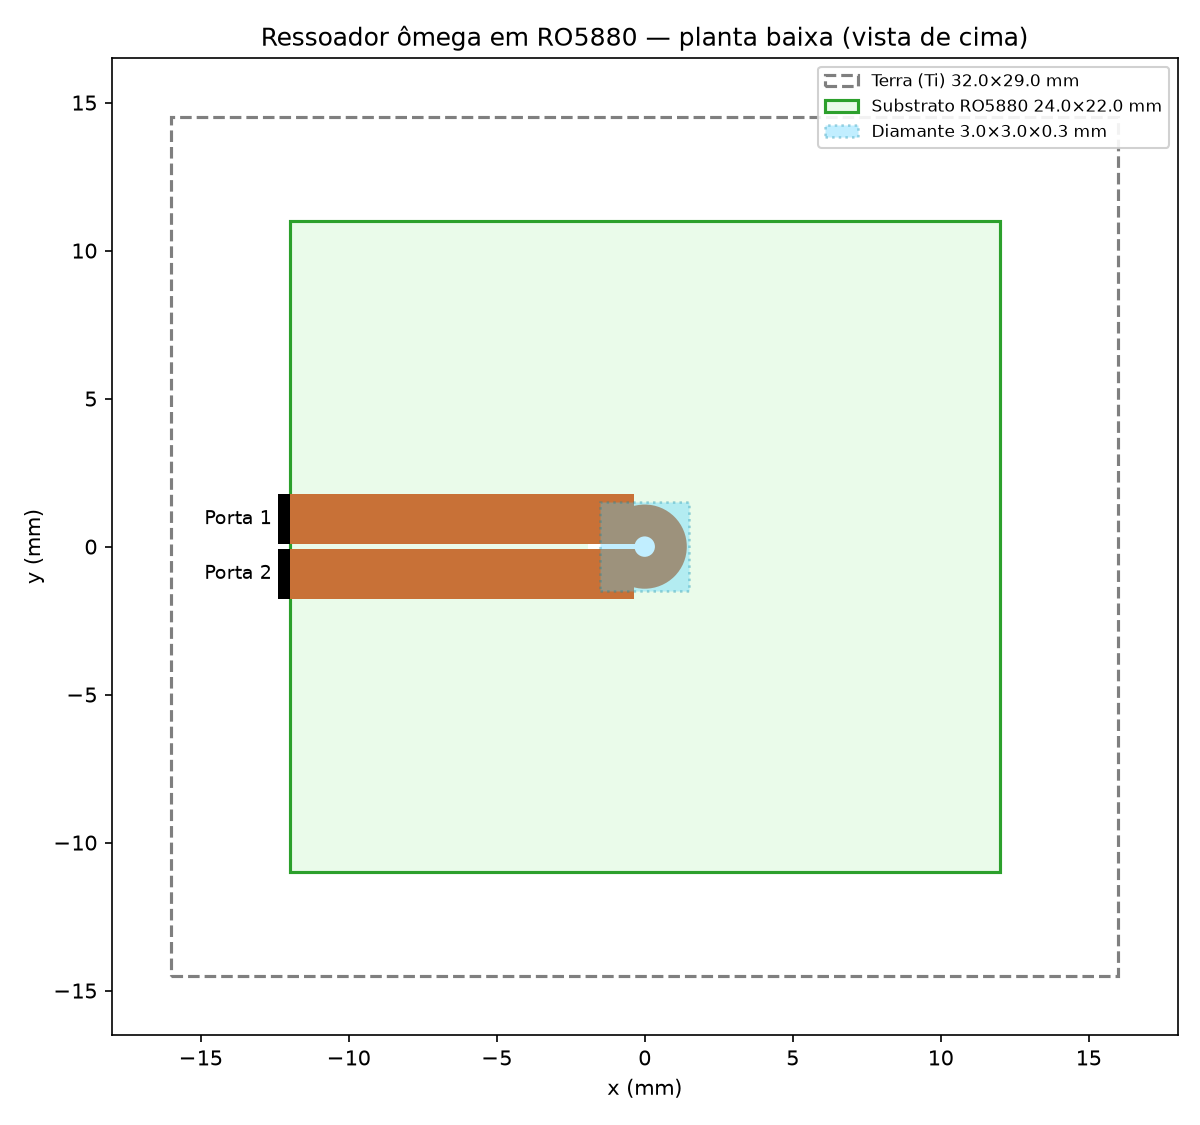
\includegraphics[width=0.75\textwidth]{../results/figures/fig_planta_baixa.png}
	\legend{Fonte: elaborado pelo autor a partir dos par\^ametros exatos do modelo HFSS.}
\end{figure}

\begin{figure}[htb]
	\caption{Detalhe da abertura e da fenda capacitiva, com todas as
	cotas e amplia\c{c}\~ao da fenda de 0,15\,mm.}
	\label{fig:detalhe-abertura}
	\centering
	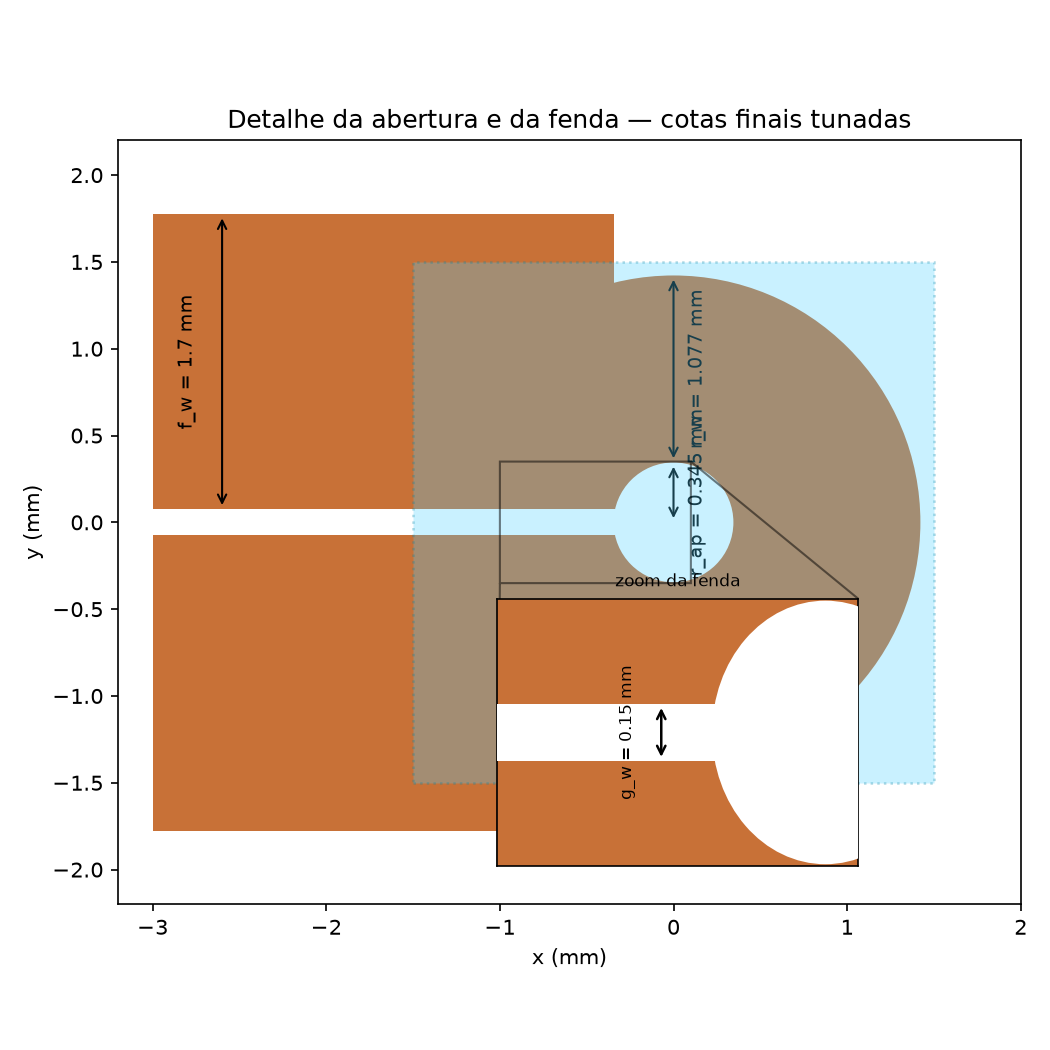
\includegraphics[width=0.7\textwidth]{../results/figures/fig_detalhe_abertura.png}
	\legend{Fonte: elaborado pelo autor.}
\end{figure}

\begin{figure}[htb]
	\caption{Corte lateral da pilha de materiais (terra de Ti, substrato
	RO5880, condutor, diamante). Escala vertical exagerada para
	clareza.}
	\label{fig:stackup}
	\centering
	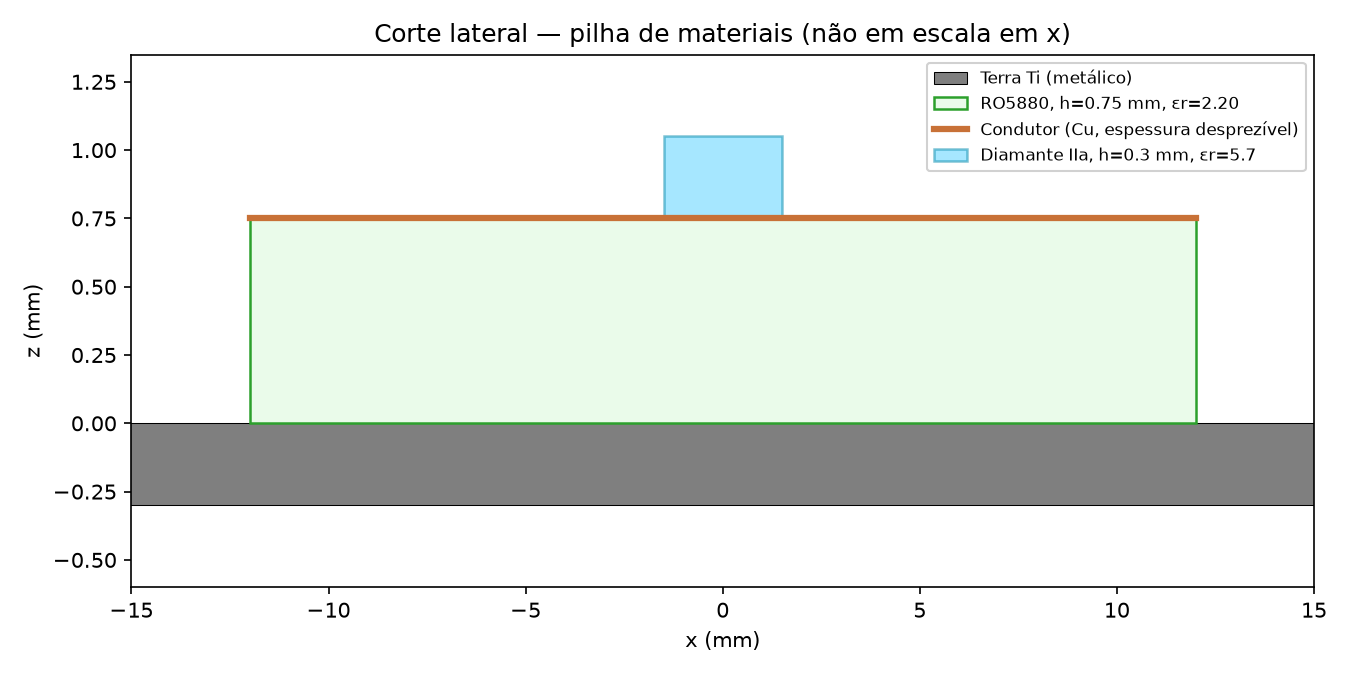
\includegraphics[width=0.85\textwidth]{../results/figures/fig_stackup_lateral.png}
	\legend{Fonte: elaborado pelo autor.}
\end{figure}

\begin{figure}[htb]
	\caption{Vista isom\'etrica do modelo, exportada diretamente do
	Ansys HFSS (\texttt{export\_model\_picture}).}
	\label{fig:hfss-iso}
	\centering
	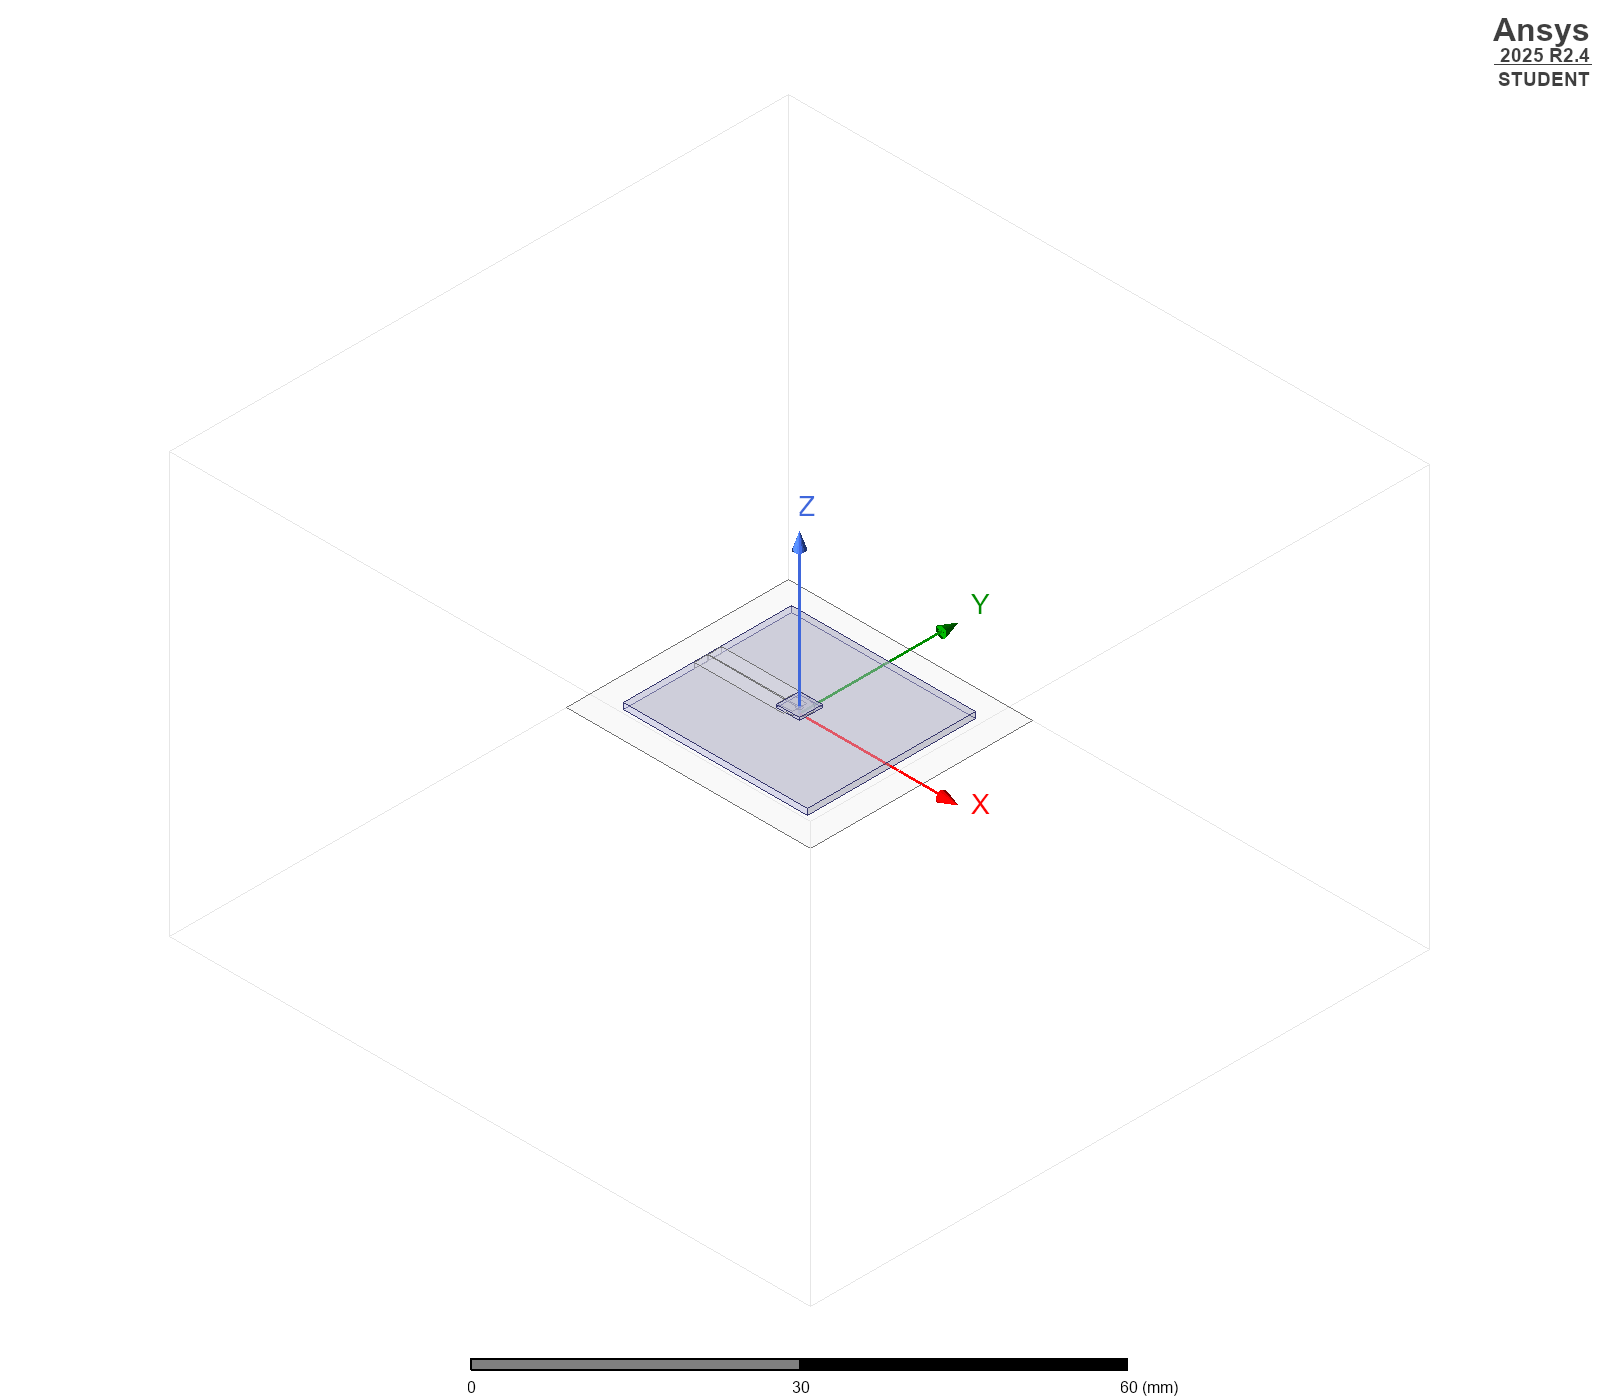
\includegraphics[width=0.75\textwidth]{../results/figures/fig_hfss_isometrica.png}
	\legend{Fonte: Ansys HFSS 2025~R2 Student, modelo simulado.}
\end{figure}

\begin{figure}[htb]
	\caption{Vista de topo do modelo, exportada diretamente do
	Ansys HFSS.}
	\label{fig:hfss-top}
	\centering
	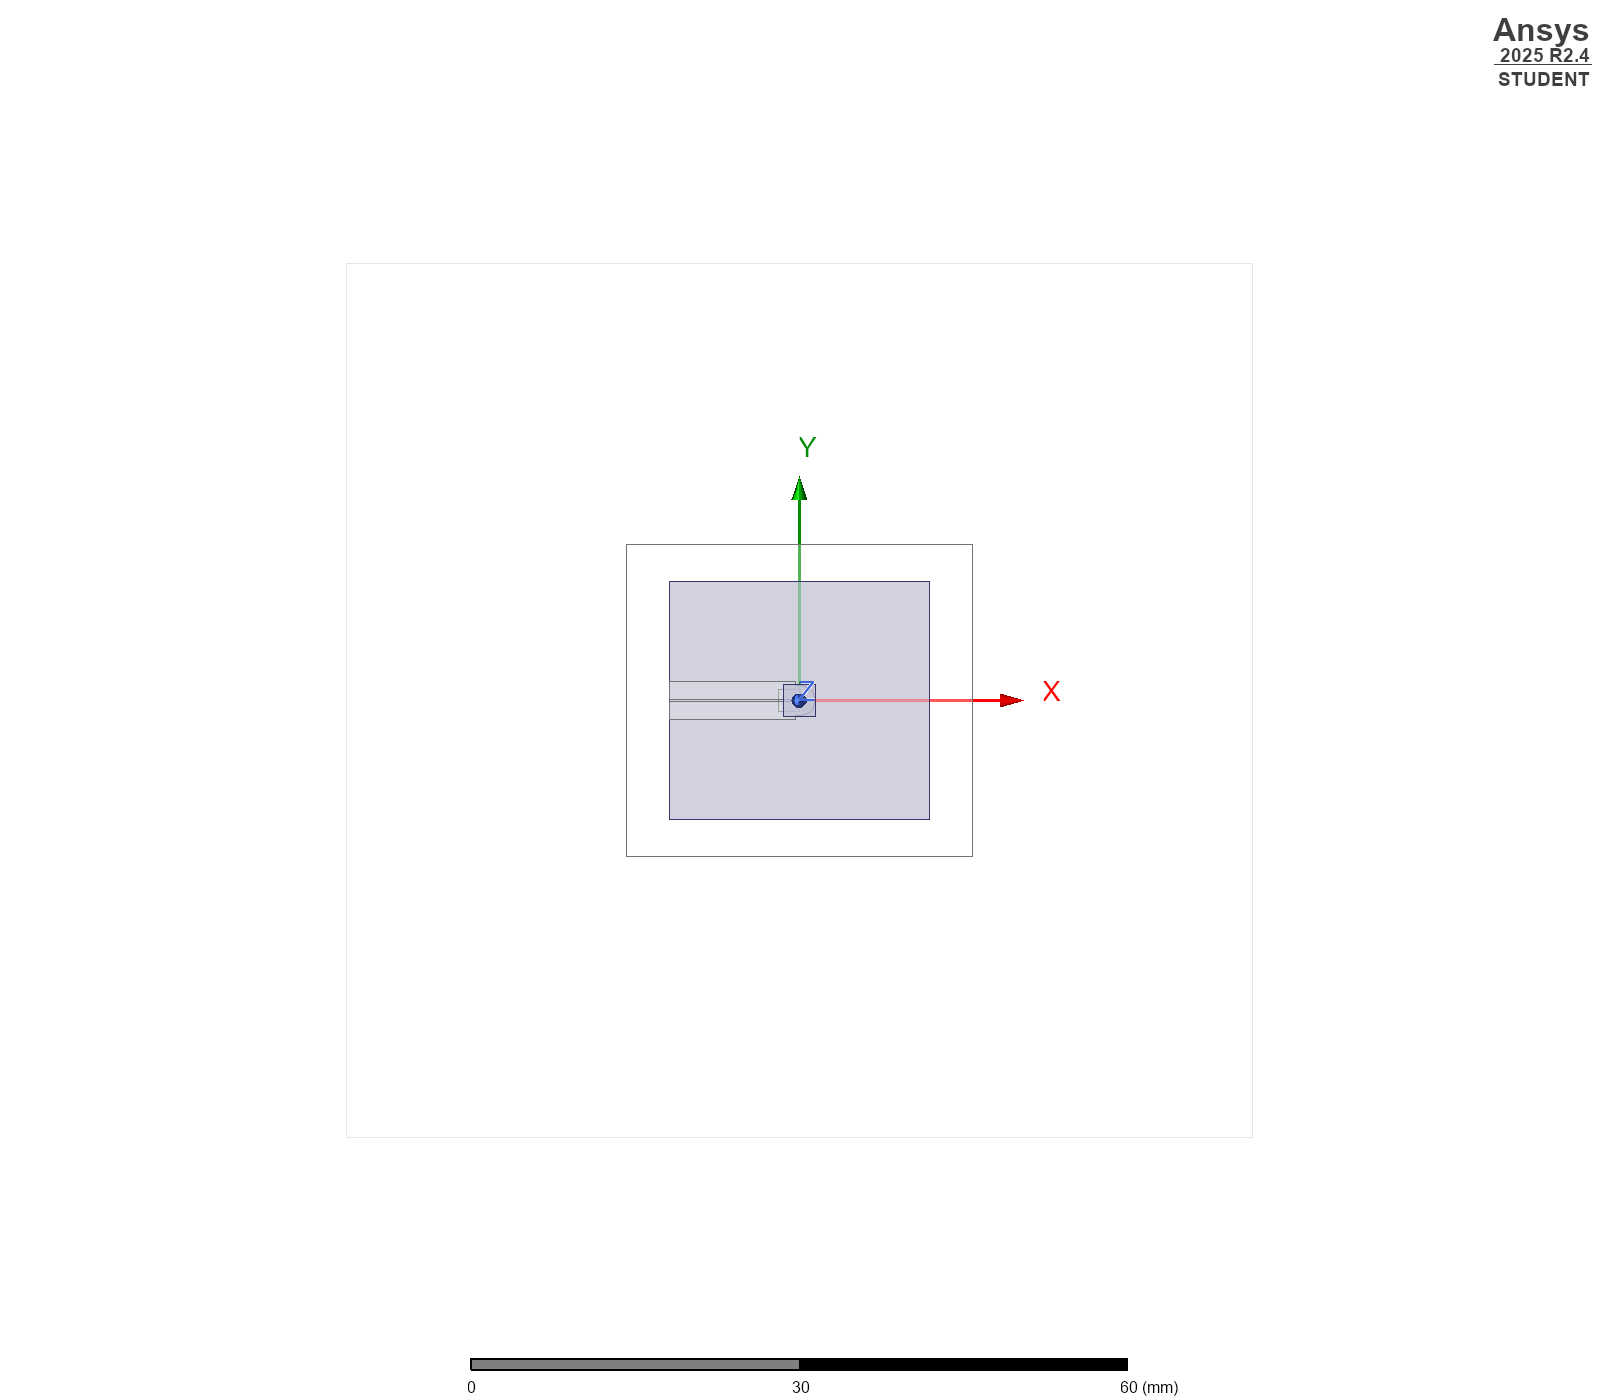
\includegraphics[width=0.75\textwidth]{../results/figures/fig_hfss_topo.png}
	\legend{Fonte: Ansys HFSS 2025~R2 Student, modelo simulado.}
\end{figure}

\begin{figure}[htb]
	\caption{Vista 3D ilustrativa completa da estrutura (reconstru\c{c}\~ao
	fiel a partir dos par\^ametros exatos do modelo, usada porque a vista
	nativa do HFSS na escala da placa inteira n\~ao resolve o detalhe da
	abertura).}
	\label{fig:3d-completa}
	\centering
	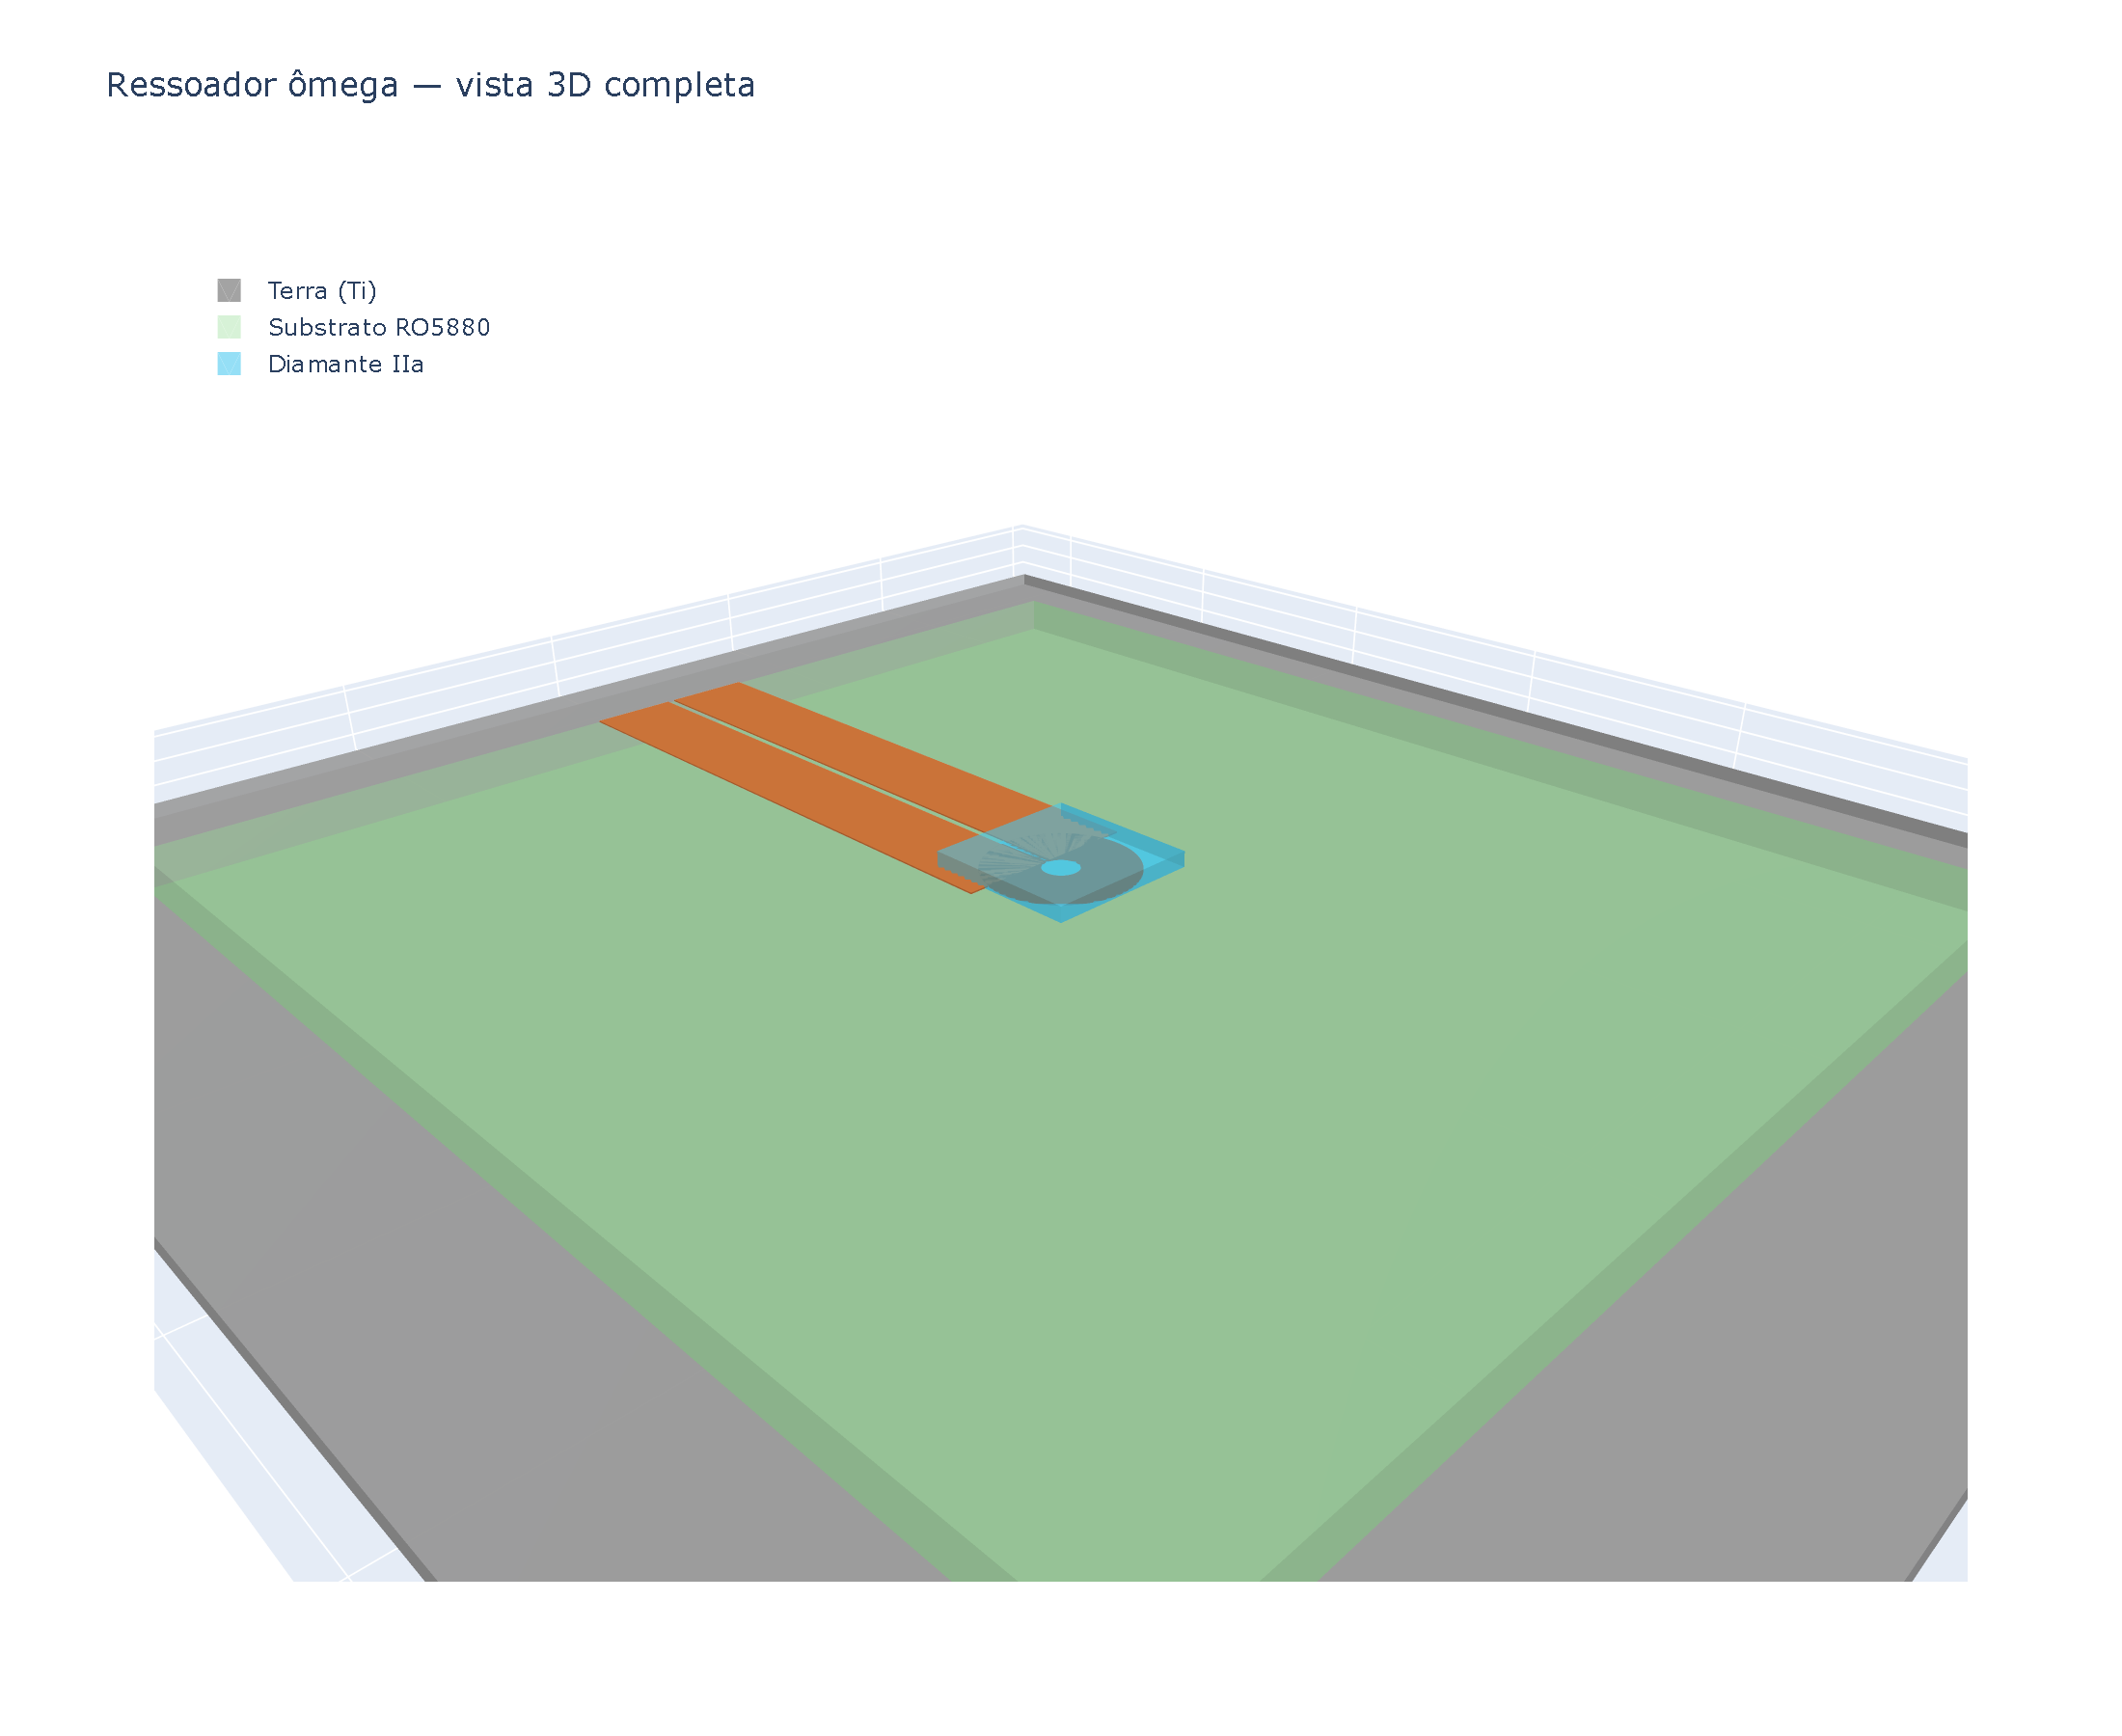
\includegraphics[width=0.75\textwidth]{../results/figures/fig_3d_estrutura_completa.png}
	\legend{Fonte: elaborado pelo autor (Plotly), a partir dos par\^ametros exatos do modelo HFSS.}
\end{figure}

\begin{figure}[htb]
	\caption{Vista 3D ilustrativa em detalhe da abertura, do la\c{c}o e
	do diamante sobreposto.}
	\label{fig:3d-detalhe}
	\centering
	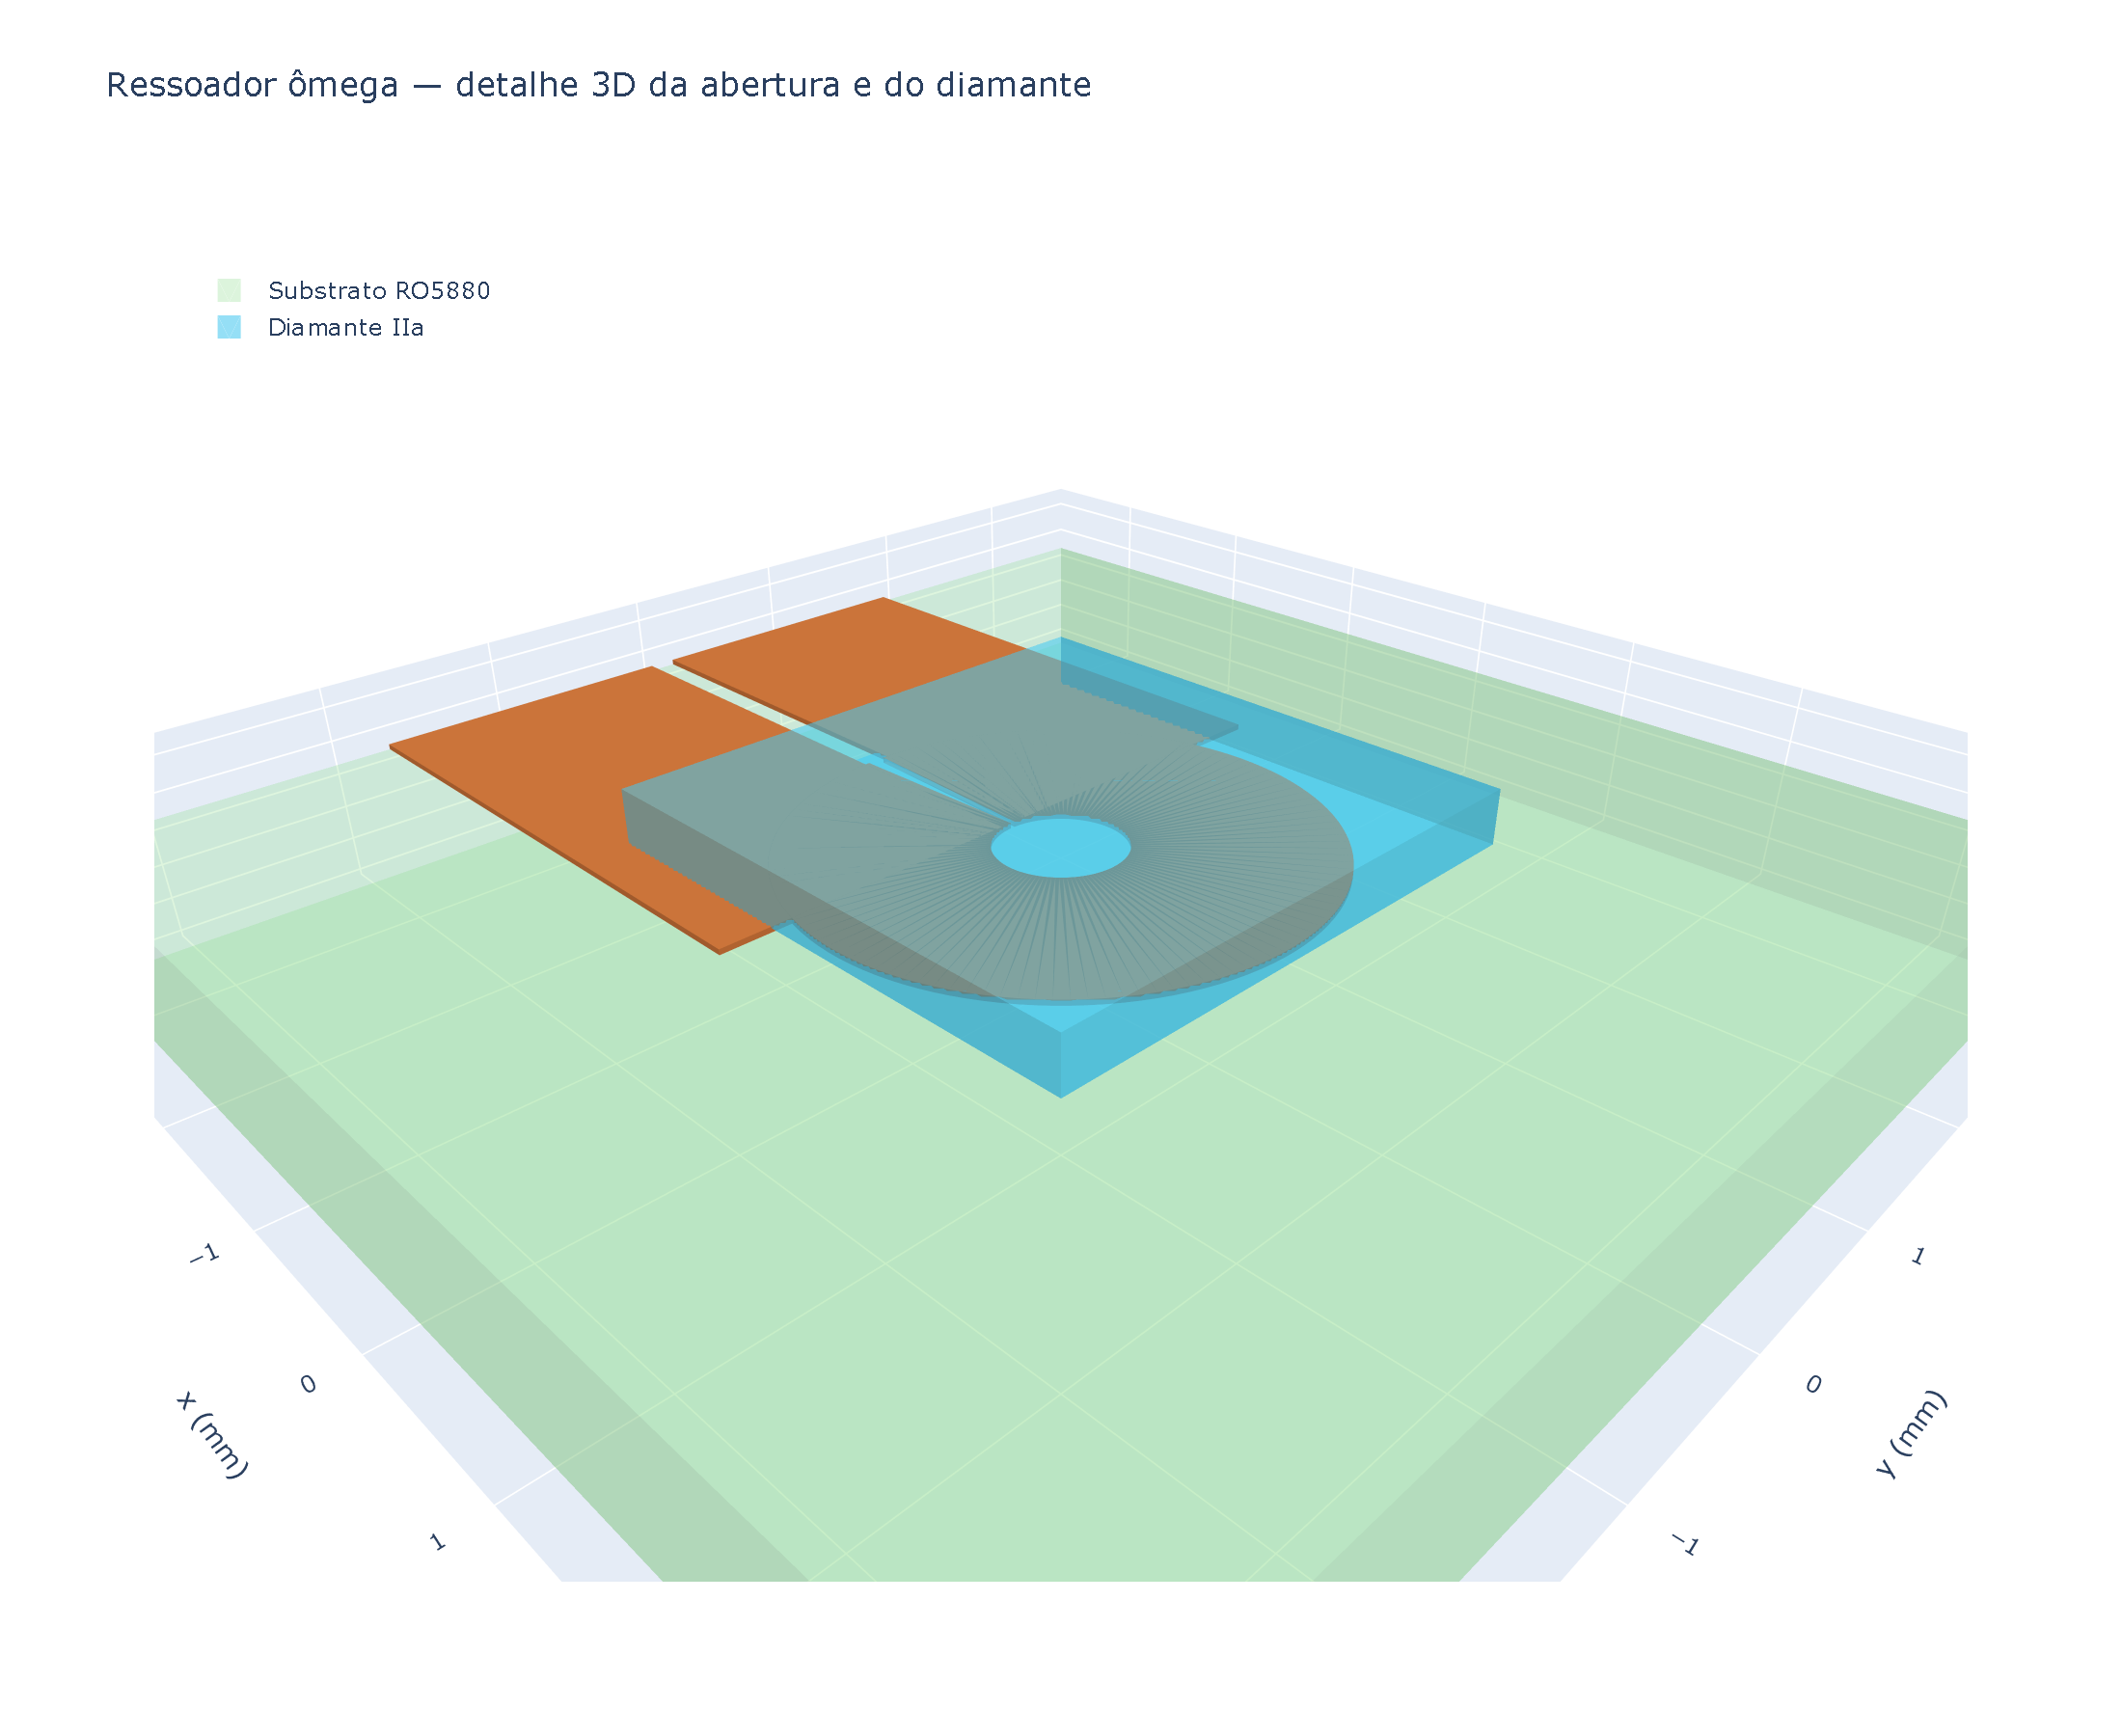
\includegraphics[width=0.7\textwidth]{../results/figures/fig_3d_detalhe_abertura.png}
	\legend{Fonte: elaborado pelo autor (Plotly).}
\end{figure}

\subsection{Par\^ametros S}

A Tabela~\ref{tab:s11} apresenta o coeficiente de reflex\~ao $S_{11}$
nos pontos de interesse, obtido pela varredura discreta verificada
(Se\c{c}\~ao~\ref{subsec:verificacao}), para tr\^es configura\c{c}\~oes:
sem diamante, com o diamante de prova, e com o diamante \textbf{e} a
alumina (superstrato, $25\times25\times0,67\,mm$,
$\varepsilon_r\approx9.8$) sobrepostos. As Figuras~\ref{fig:s11} e
\ref{fig:s21} mostram as curvas completas na banda
2,5--3,2\,GHz.

\begin{table}[htb]
	\caption{Coeficiente de reflex\~ao $S_{11}$ verificado nas
	frequ\^encias de interesse, para as tr\^es configura\c{c}\~oes de
	carregamento.}
	\label{tab:s11}
	\centering
	\begin{tabular}{lrrr}
		\toprule
		Frequ\^encia & sem diamante (dB) & com diamante (dB) & diamante+alumina (dB) \\
		\midrule
		2,50\,GHz & -27,56 & -32,26 & -17,71 \\
		2,74\,GHz ($m_s{=}0{\leftrightarrow}{-1}$) & -27,39 & -31,80 & -17,46 \\
		2,87\,GHz (ZFS do NV$^-$) & -27,42 & -31,61 & -17,43 \\
		2,97\,GHz ($m_s{=}0{\leftrightarrow}{+1}$) & -27,50 & -31,52 & -17,47 \\
		3,20\,GHz & -27,89 & -31,42 & -17,74 \\
		\bottomrule
	\end{tabular}
	\legend{Fonte: elaborado pelo autor, dados do sweep discreto do Ansys HFSS.}
\end{table}

\begin{figure}[htb]
	\caption{$S_{11}$ verificado (varredura discreta) na banda de
	interesse, para as tr\^es configura\c{c}\~oes, com as
	transi\c{c}\~oes Zeeman marcadas.}
	\label{fig:s11}
	\centering
	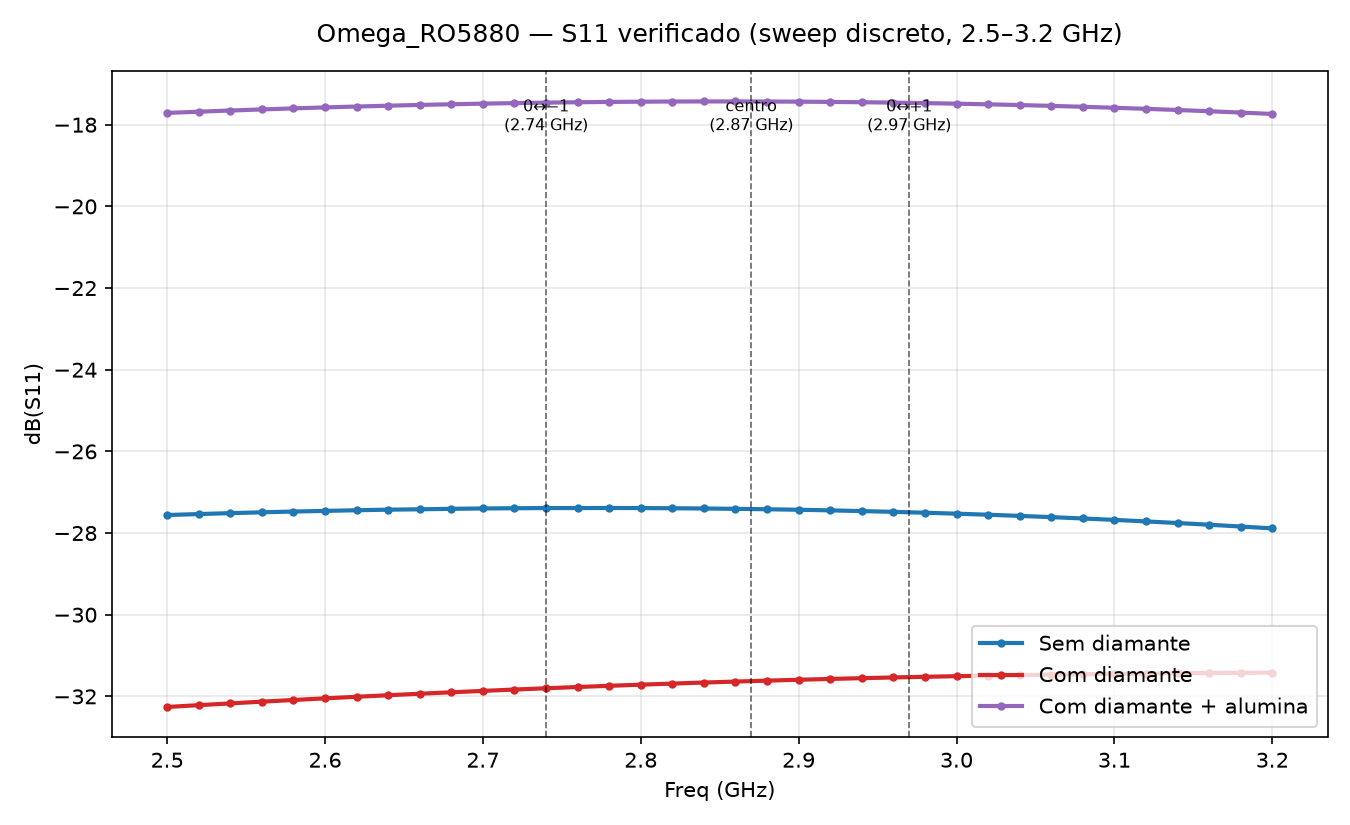
\includegraphics[width=0.9\textwidth]{../results/figures/fig_S11.png}
	\legend{Fonte: elaborado pelo autor, dados do Ansys HFSS.}
\end{figure}

\begin{figure}[htb]
	\caption{$S_{21}$ verificado na banda de interesse -- perda de
	inser\c{c}\~ao muito baixa ($<0,04\,dB$), coerente com um
	elemento de dois portos em linha.}
	\label{fig:s21}
	\centering
	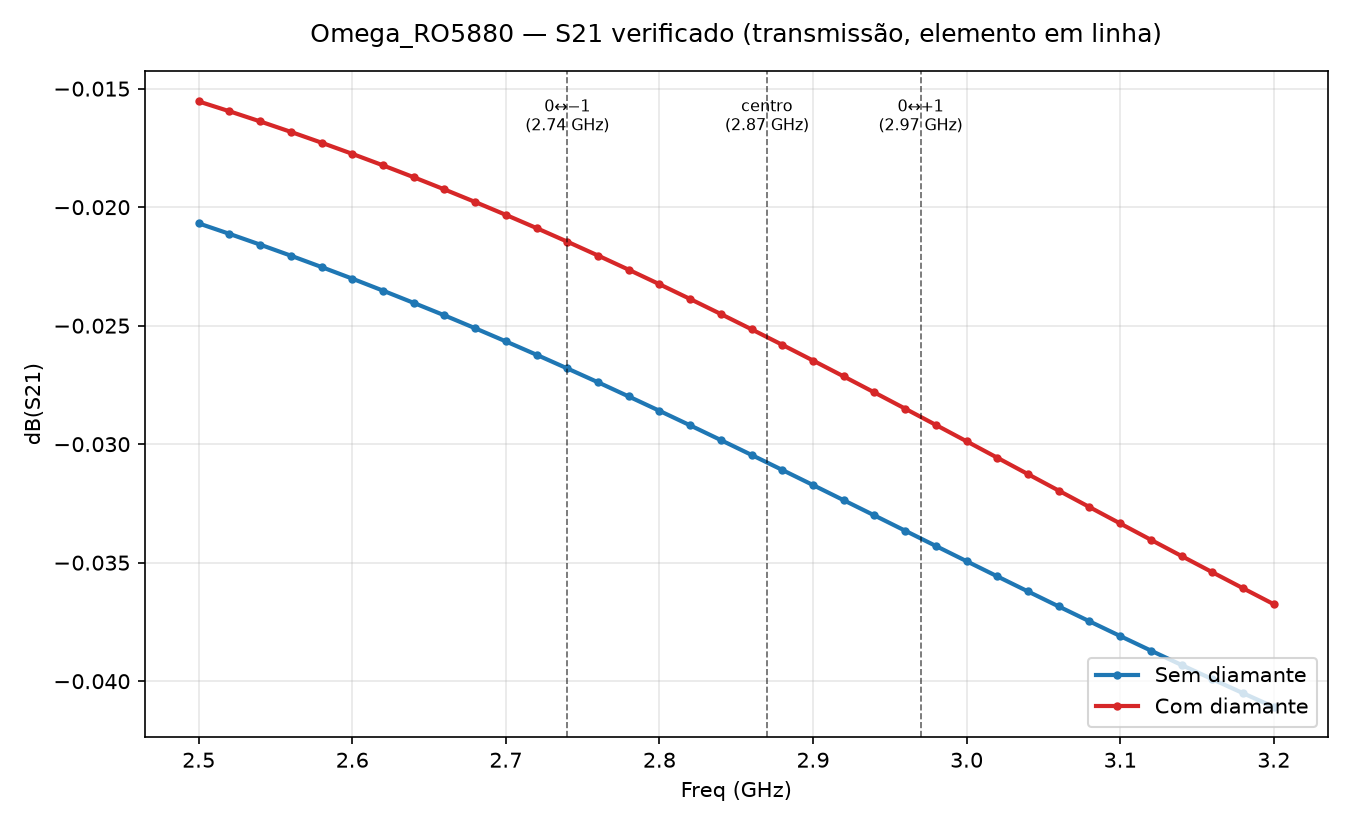
\includegraphics[width=0.9\textwidth]{../results/figures/fig_S21.png}
	\legend{Fonte: elaborado pelo autor, dados do Ansys HFSS.}
\end{figure}

\begin{figure}[htb]
	\caption{Efeito do carregamento diel\'etrico do diamante sobre o
	casamento -- deslocamento $\Delta S_{11}$ negativo (melhora) em toda
	a banda.}
	\label{fig:delta}
	\centering
	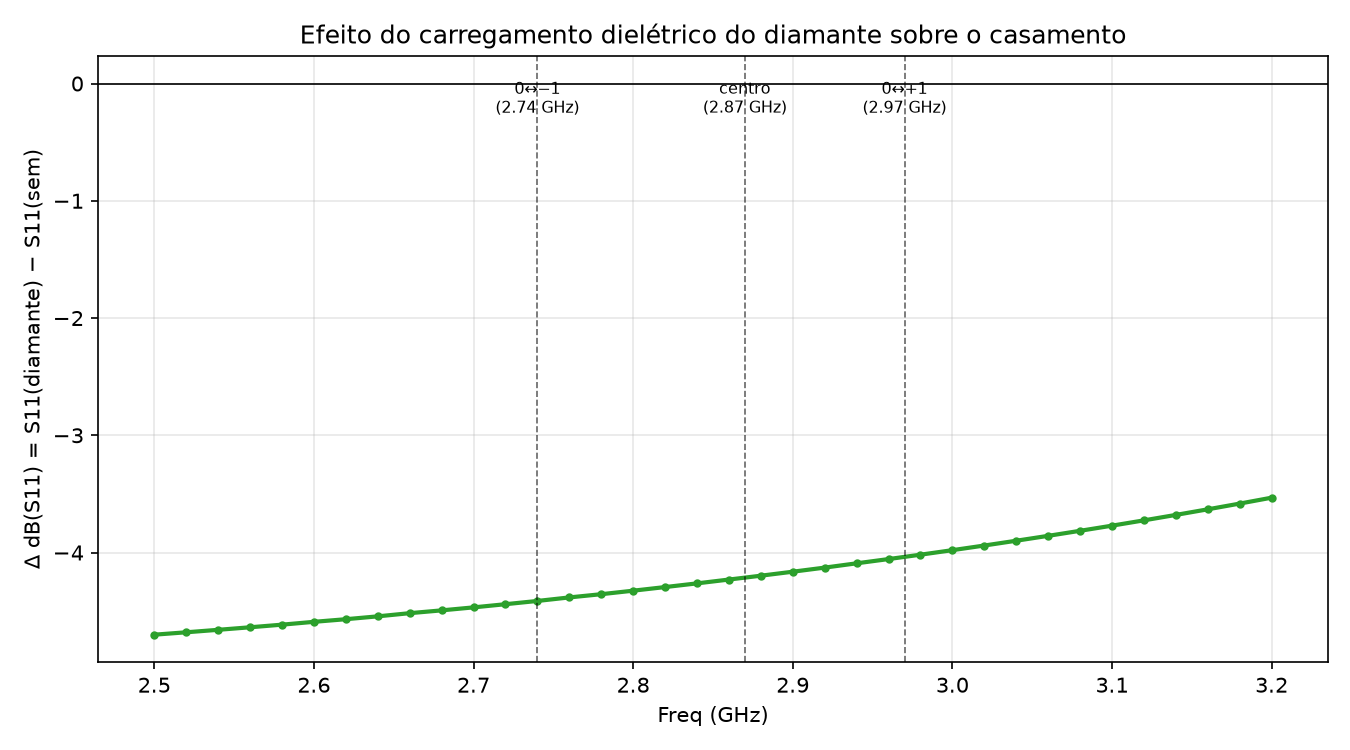
\includegraphics[width=0.85\textwidth]{../results/figures/fig_delta_diamante.png}
	\legend{Fonte: elaborado pelo autor, dados do Ansys HFSS.}
\end{figure}

\subsection{Campo magn\'etico pr\'oximo}
\label{subsec:campos}

A figura de m\'erito real do projeto -- n\~ao o $S_{11}$, mas o campo
magn\'etico $B_1$ dentro da abertura (Se\c{c}\~ao~\ref{sec:introducao})
-- foi avaliada por dois cortes de linha (eixos $x$ e $y$, $\pm2\,mm$)
passando pelo centro da abertura, na altura do topo do diamante, no
design \texttt{Omega\_RO5880\_Diamond}, replicando a metodologia dos
cortes de linha da Fig.~4 de \citeonline{opaluch2021}.

\begin{table}[htb]
	\caption{Magnitude do campo $H$ dentro da abertura ($1$~W na
	porta), nos dois cortes de linha.}
	\label{tab:campo}
	\centering
	\begin{tabular}{lrrrr}
		\toprule
		Corte & m\'inimo (A/m) & m\'aximo (A/m) & m\'edia (A/m) & varia\c{c}\~ao (\%) \\
		\midrule
		$x$ (paralelo ao gap)      & 41,6 & 62,3 & 57,0 & 36,3 \\
		$y$ (perpendicular ao gap) & 45,9 & 62,5 & 58,3 & 28,5 \\
		\bottomrule
	\end{tabular}
	\legend{Fonte: elaborado pelo autor, dados do Ansys HFSS (relat\'orio de campo em linha).}
\end{table}

\begin{figure}[htb]
	\caption{Magnitude do campo $H$ ao longo dos dois cortes de linha,
	$1$~W na porta, 2,87\,GHz.}
	\label{fig:campo}
	\centering
	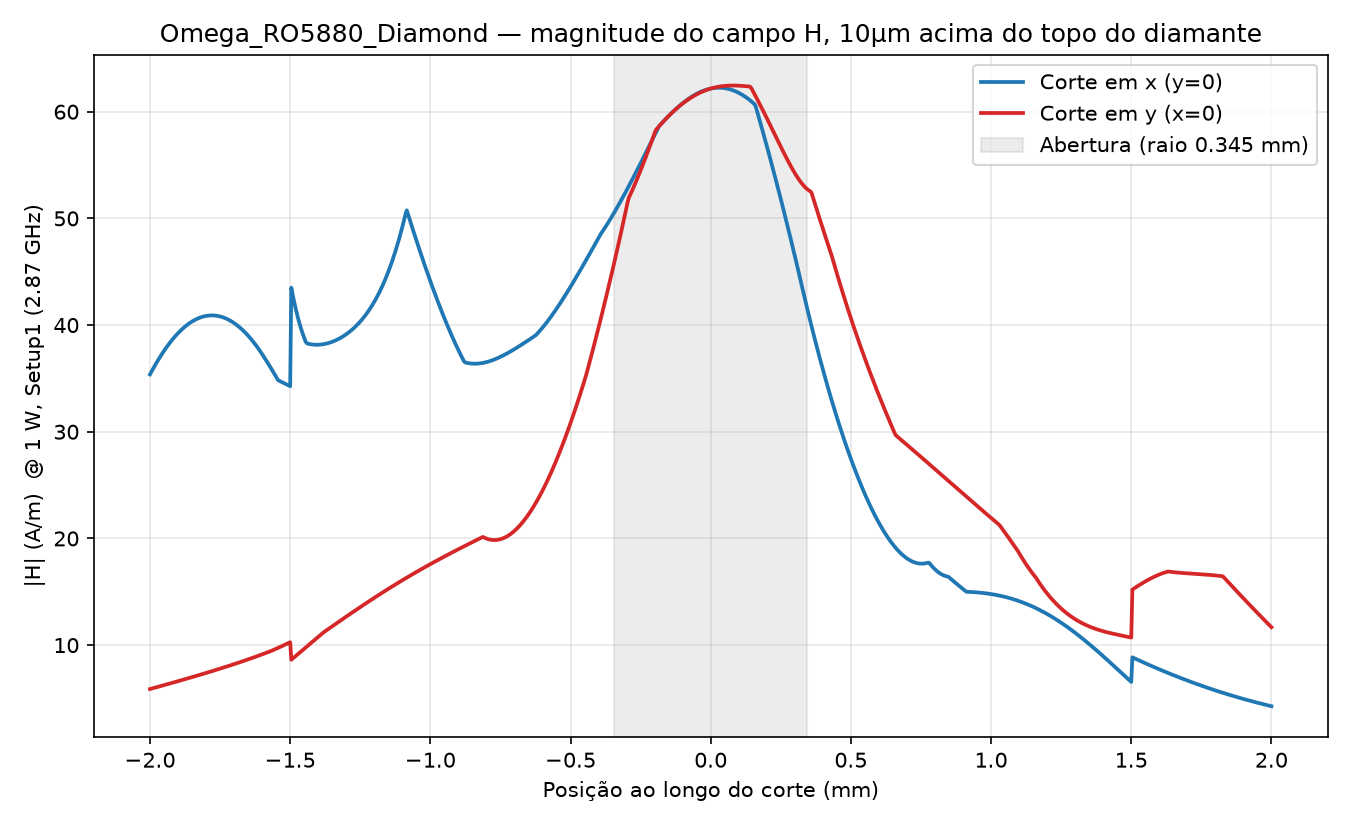
\includegraphics[width=0.85\textwidth]{../results/figures/fig_campo_MagH_cortes.png}
	\legend{Fonte: elaborado pelo autor, dados do Ansys HFSS.}
\end{figure}

O campo \'e m\'aximo ($\approx62\,A/m$ a 1\,W) muito
pr\'oximo do centro da abertura e decai monotonicamente para fora
(Figura~\ref{fig:campo}), com uma assimetria real entre os dois
cortes -- esperada, j\'a que o gap capacitivo (situado no eixo $-x$)
quebra a simetria azimutal da estrutura, o mesmo tipo de assimetria
relatada por \citeonline{opaluch2021} entre os cortes paralelo e
perpendicular ao gap. As pequenas discontinuidades em
$x,y=\pm1,5\,mm$ coincidem com a borda do diamante
($3\times3\,mm$), consistentes com uma transi\c{c}\~ao de
malha na interface de material. A ordem de grandeza \'e compar\'avel \`a
refer\^encia, por\'em menor -- \citeonline{opaluch2021} relatam
170--280\,A/m a 1\,W para a geometria original (gap de
7\,\textmu m, litografia); aqui, com um gap de PCB
(150\,\textmu m, cerca de $20\times$ maior) e geometria
reotimizada, o elemento capacitivo \'e proporcionalmente mais fraco,
explicando o campo menor.

\textbf{A componente perpendicular ($H_z$) n\~ao foi extra\'ida
numericamente.} Diversas tentativas de isolar essa componente --
tanto pela calculadora de campos do \emph{pyaedt} (produto escalar com
vetor unit\'ario $\hat{z}$, opera\c{c}\~ao \texttt{ScalarZ}) quanto por
express\~oes nomeadas de relat\'orio (\texttt{Hz}, \texttt{Mag\_Hz})
-- encontraram incompatibilidades reais na vers\~ao instalada do
\emph{pyaedt} (1.6.0): erros de execu\c{c}\~ao remota
(\texttt{GrpcApiError}) ou aus\^encia de dados retornada sem detalhe
adicional. Apenas a magnitude do vetor completo (\texttt{Mag\_H}),
apresentada acima, p\^ode ser extra\'ida de forma confi\'avel. A
predomin\^ancia da componente perpendicular pr\'oxima ao centro,
entretanto, \'e uma consequ\^encia direta de simetria em
magnetost\'atica -- o campo no eixo de um la\c{c}o de corrente circular
\'e puramente axial --, e a pr\'opria refer\^encia confirma essa
predomin\^ancia dentro de um raio de $\approx260\,\textmu m$ para
geometria semelhante \cite{opaluch2021}; a expectativa f\'isica \'e,
portanto, s\'olida mesmo sem confirma\c{c}\~ao num\'erica direta nesta
vers\~ao do \emph{software}. Uma confirma\c{c}\~ao visual direta pelo
gerador de gr\'aficos de campo do pr\'oprio HFSS (\emph{Fields~$>$~Plot
Fields}), n\~ao dependente de \emph{scripting}, permanece como
verifica\c{c}\~ao recomendada (Se\c{c}\~ao~\ref{sec:trabalhos-futuros}).

\subsection{Discuss\~ao}

O casamento obtido \'e uma \textbf{cauda larga e suave}, n\~ao um pico
estreito de alto fator de qualidade -- a resson\^ancia mais profunda do
la\c{c}o situa-se pr\'oxima de ou abaixo de 0,5\,GHz, e o
que se observa na banda de 2,5--3,2\,GHz \'e a cauda
dessa resson\^ancia. Esse comportamento atende exatamente ao requisito
f\'isico do projeto (Se\c{c}\~ao~\ref{sec:introducao}): banda m\'inima
de 250\,MHz cobrindo as duas transi\c{c}\~oes Zeeman sem necessidade de reajuste. A profundidade obtida ($-27$ a $-32$~dB, ou seja, no m\'aximo
$\approx0.2\%$ da pot\^encia incidente refletida) \'e da mesma ordem de
grandeza da relatada no artigo de refer\^encia ($-47$~dB em um \'unico
ponto), com a diferen\c{c}a absoluta esperada dado que a geometria foi
inteiramente reotimizada para os materiais e o processo de fabrica\c{c}\~ao
dispon\'iveis, em vez de reproduzir as dimens\~oes de litografia do
artigo original.

Um resultado notavelmente positivo foi o efeito do diamante de prova
sobre o casamento (Figura~\ref{fig:delta}): em vez de deslocar o
ressoador para fora da banda de projeto -- risco t\'ipico de um
carregamento diel\'etrico sobre uma resson\^ancia estreita --, o
diamante deslocou o $S_{11}$ para valores \emph{mais profundos}
($\approx-4.4$~dB adicionais) em toda a banda de interesse. Isso
confirma, empiricamente, a expectativa te\'orica que motivou a escolha
de um casamento de banda larga: sua robust\^ez a perturba\c{c}\~oes de
carregamento moderadas.

Adicionar a alumina sobre o diamante, por outro lado, deslocou o
casamento para valores menos favor\'aveis ($\approx-31$~dB para $\approx-17$~dB,
Tabela~\ref{tab:s11}) -- um carregamento diel\'etrico maior (placa de
$25\times25\,mm$, $\varepsilon_r\approx9.8$, contra o
diamante de $3\times3\,mm$, $\varepsilon_r=5.7$) desloca o
ressoador mais para fora do seu ponto \'otimo. Ainda assim, o
casamento permanece \textbf{bem funcional} ($-17$~dB, ou seja
$\approx2\%$ de pot\^encia refletida, abaixo do limiar usual de
$-10$~dB, adotado como refer\^encia de bom casamento em projetos de
RF), e preserva a mesma forma de cauda larga -- n\~ao houve nenhum
deslocamento cat\'astrofico para fora da banda de interesse, o que
seria de se esperar caso o casamento original fosse um pico estreito
de alto fator de qualidade em vez de banda larga.

\section{Conclus\~ao e trabalhos futuros}
\label{sec:trabalhos-futuros}

O ressoador \^omega de dois portos foi projetado com sucesso para os
materiais dispon\'iveis (Rogers RT/duroid~5880, diamante IIa e
alumina), atingindo casamento de banda larga verificado
($S_{11} \leq -17$~dB com todas as cargas, $\leq -27$~dB sem alumina,
em toda a banda 2,5--3,2\,GHz) por dois m\'etodos
num\'ericos independentes, com todas as dimens\~oes do condutor
compat\'iveis com processo convencional de PCB. Os pr\'oximos passos
do projeto, em ordem de prioridade, s\~ao:

\begin{enumerate}
	\item \textbf{Confirmar com o orientador a suposi\c{c}\~ao do plano
	de terra} (Se\c{c}\~ao~\ref{sec:fundamentacao}): titan\^io n\~ao
	consta na lista de materiais confirmados como dispon\'iveis --
	essa dimens\~ao e material foram copiados do \emph{setup} do
	artigo de refer\^encia sem verifica\c{c}\~ao. Todos os resultados
	de $S_{11}$ deste relat\'orio dependem dessa suposi\c{c}\~ao;
	\item \textbf{Confirmar a extra\c{c}\~ao num\'erica da componente
	perpendicular ($H_z$)} do campo magn\'etico, seja atualizando o
	\emph{pyaedt} para uma vers\~ao sem a incompatibilidade descrita na
	Se\c{c}\~ao~\ref{subsec:campos}, seja por inspe\c{c}\~ao visual
	direta no gerador de gr\'aficos de campo do pr\'oprio HFSS
	(n\~ao dependente de \emph{scripting});
	\item Ajuste fino de $f_w$ para casamento pr\'oximo de
	50\,$\Omega$ nas linhas de alimenta\c{c}\~ao, caso necess\'ario
	para a interface com a instrumenta\c{c}\~ao de micro-ondas;
	\item Confirmar com o orientador o papel exato da alumina no
	experimento (superstrato de prote\c{c}\~ao? suporte de amostra?
	outra fun\c{c}\~ao?) -- a simula\c{c}\~ao atual trata-a como
	superstrato sobre o diamante, mas essa configura\c{c}\~ao ainda
	n\~ao foi confirmada como a correta.
\end{enumerate}

\clearpage
\printbibliography[heading=bibintoc,title={Refer\^encias}]

\end{document}









